\indent\indent The \textit{Relative neighbors disp.} tool offers you a powerful way to automatically clean your data.\\
\newline
\indent The algorithm will provide you a graph displaying the relative displacement of each marker compared to his closest neighbors during the whole correlation process. A marker with high displacements compared to its neighbors may be badly correlated and should be masked. You can also detect when a marker starts to behave differently compared to its neighbors.\\
\indent In order to masked the unwanted markers, move the two upper and lower red lines on the graph representing the maximum relative displacement for each marker. If a marker cross the upper or lower limit, it'll automatically be masked.\\

\begin{figure}[!h]
   \centering
   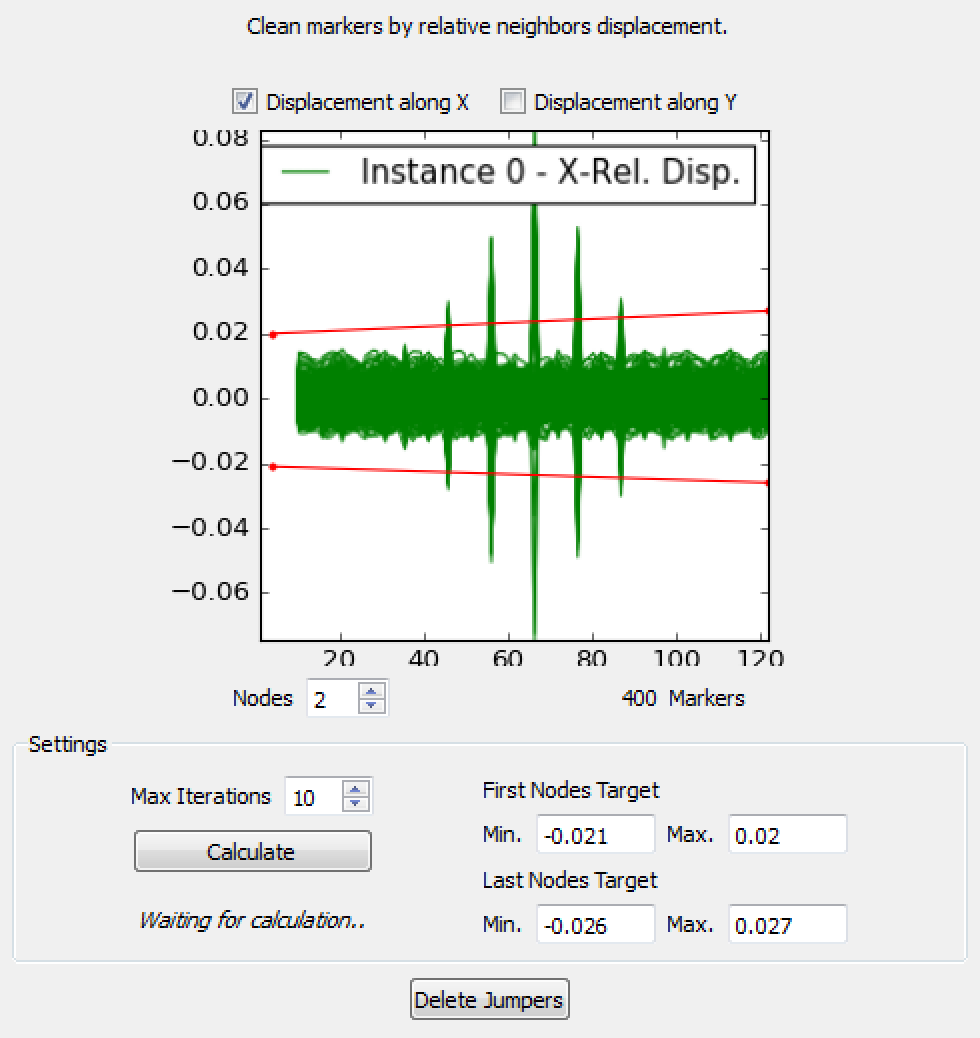
\includegraphics[scale=.6]{relative_neighbors}
   \caption{Relative Neighbors Disp. - Define upper and lower limits}
\end{figure}

\newpage
\indent A masked marker may generate new high relative displacement in the new neighborhood of some markers. The algorithm will automatically recalculate the relative displacement after a deletion and continue the cleaning if some markers are then crossing the predefined upper and lower limits. Once all the unwanted have been masked (or the iteration number is reached), the new graph is displayed and you can then confirm the calculation to apply the mask to your data or set new limits.\\
\newline
\indent When a mask is applied, the previous state of the analysis is automatically saved in the analysis folder.\\
On start-up, the software will load the last mask version by default. If you made a mistake or want to bring back your data, you can open a previous version by using the \text{Open Mask/Version} option in the \textit{File} menu.\\
\newline
\indent Please keep in mind that when a mask is applied, the data is only hidden and not modified. An older version can always be loaded.
